% ==============================================================================
% capitulos/00-anexoE.tex - Reportes Técnicos: Microservicio Quejoso
% ==============================================================================

\chapter{Reportes Técnicos: Microservicio Quejoso}
\label{anexo:reportes_quejoso}

En este anexo se presentan los reportes íntegros generados mediante el análisis estático (SAST) realizado específicamente al microservicio del Quejoso. Estos documentos sirven como evidencia técnica para las vulnerabilidades descritas en la sección de Análisis de Riesgo.

\section{Reporte de Gobernanza (Governance Report)}
\label{anexo:quejoso_gov}
Este documento detalla los indicadores de calidad del código, destacando un \textit{Global Indicator} de 90.54 y un nivel de criticidad de negocio alto.

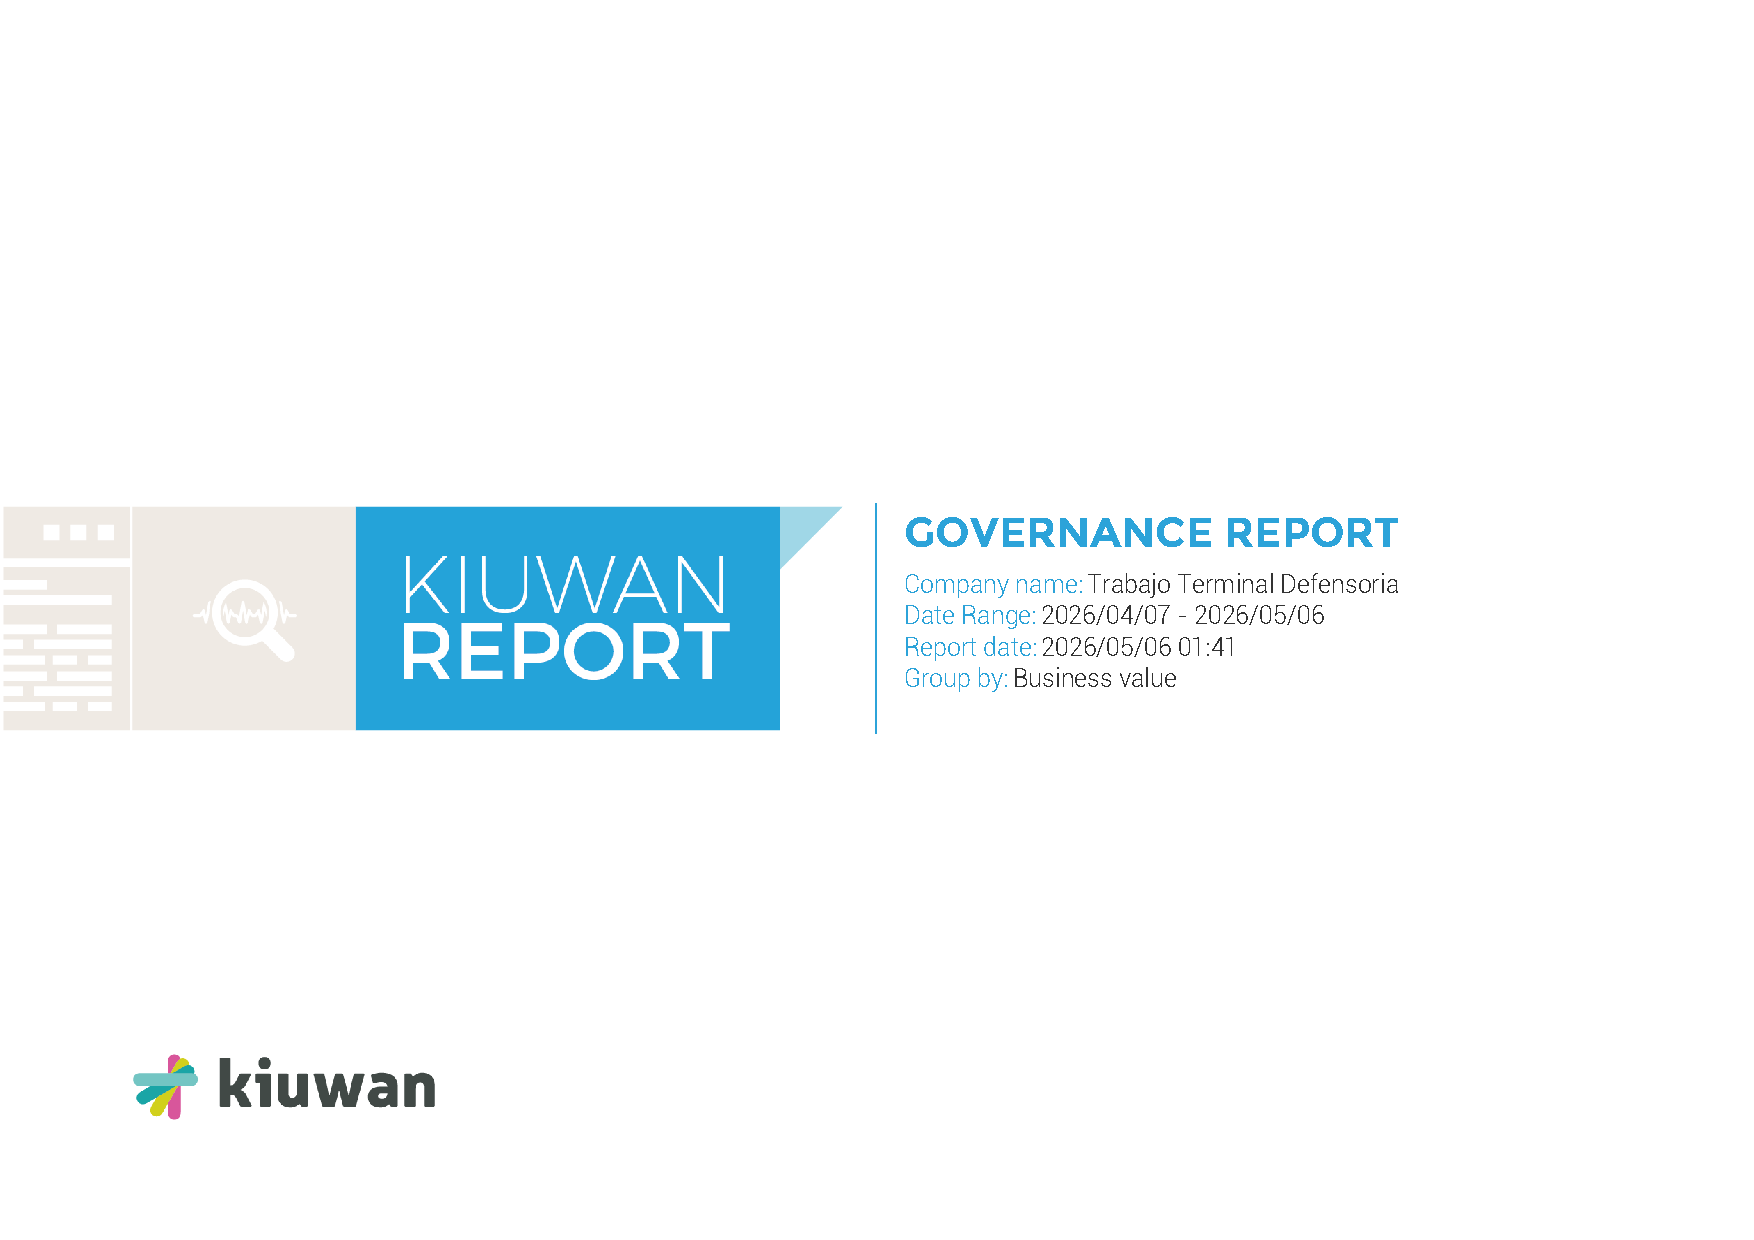
\includepdf[pages=-, frame, scale=0.8, pagecommand={\thispagestyle{plain}}]{kiuwan/quejoso/GOVERNANCE_REPORT-QUEJOSO.pdf}

\section{Análisis de Vulnerabilidades (Vulnerabilities Report)}
\label{anexo:quejoso_vuln}
Este reporte identifica los defectos de seguridad específicos, incluyendo las vulnerabilidades de inyección y criptografía débil detectadas en el código fuente de Java.

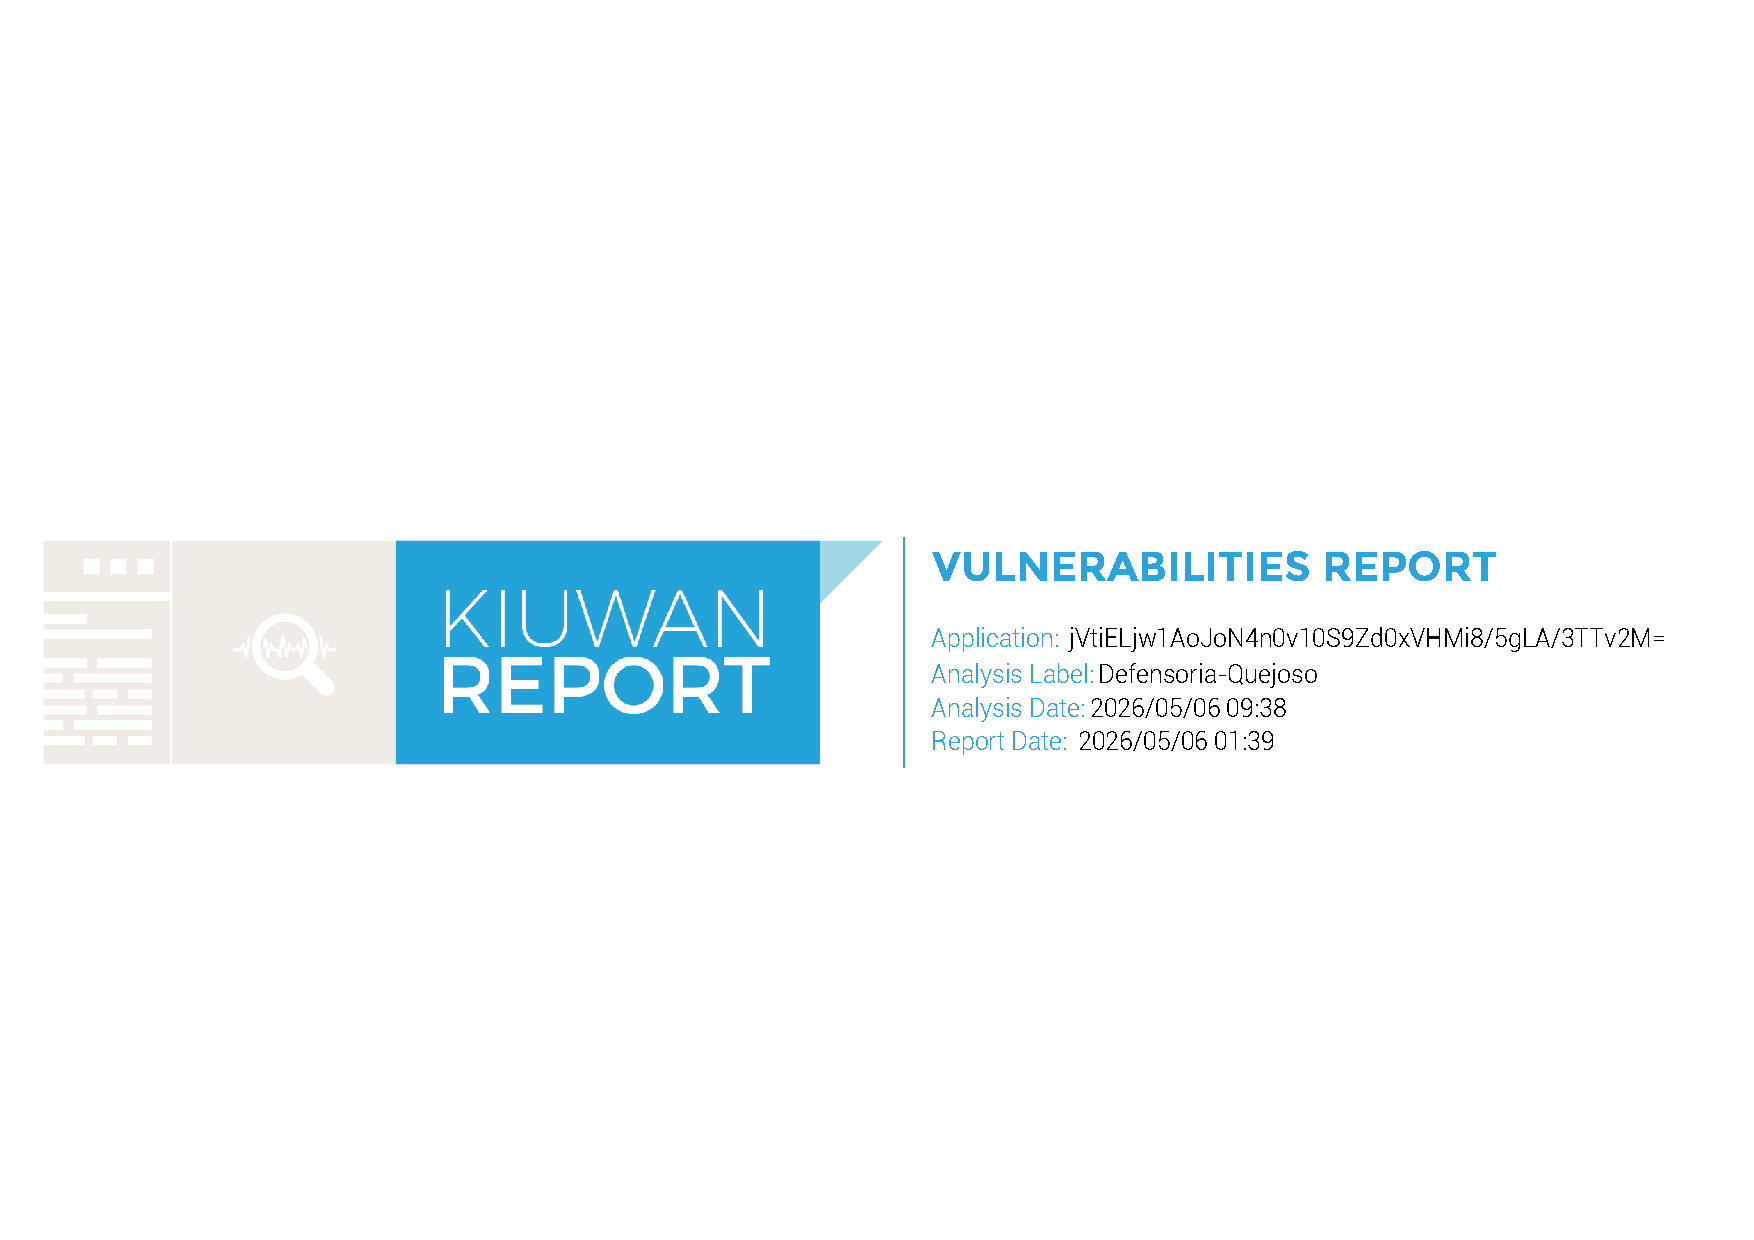
\includepdf[pages=-, frame, scale=0.8, pagecommand={\thispagestyle{plain}}]{kiuwan/quejoso/VULNERABILITIES_REPORT-QUEJOSO.pdf}

\section{Inventario de Componentes (Insights Report)}
\label{anexo:quejoso_insight}
Detalle del inventario de las 73 dependencias de terceros utilizadas por el microservicio y el análisis de su estado de obsolescencia.

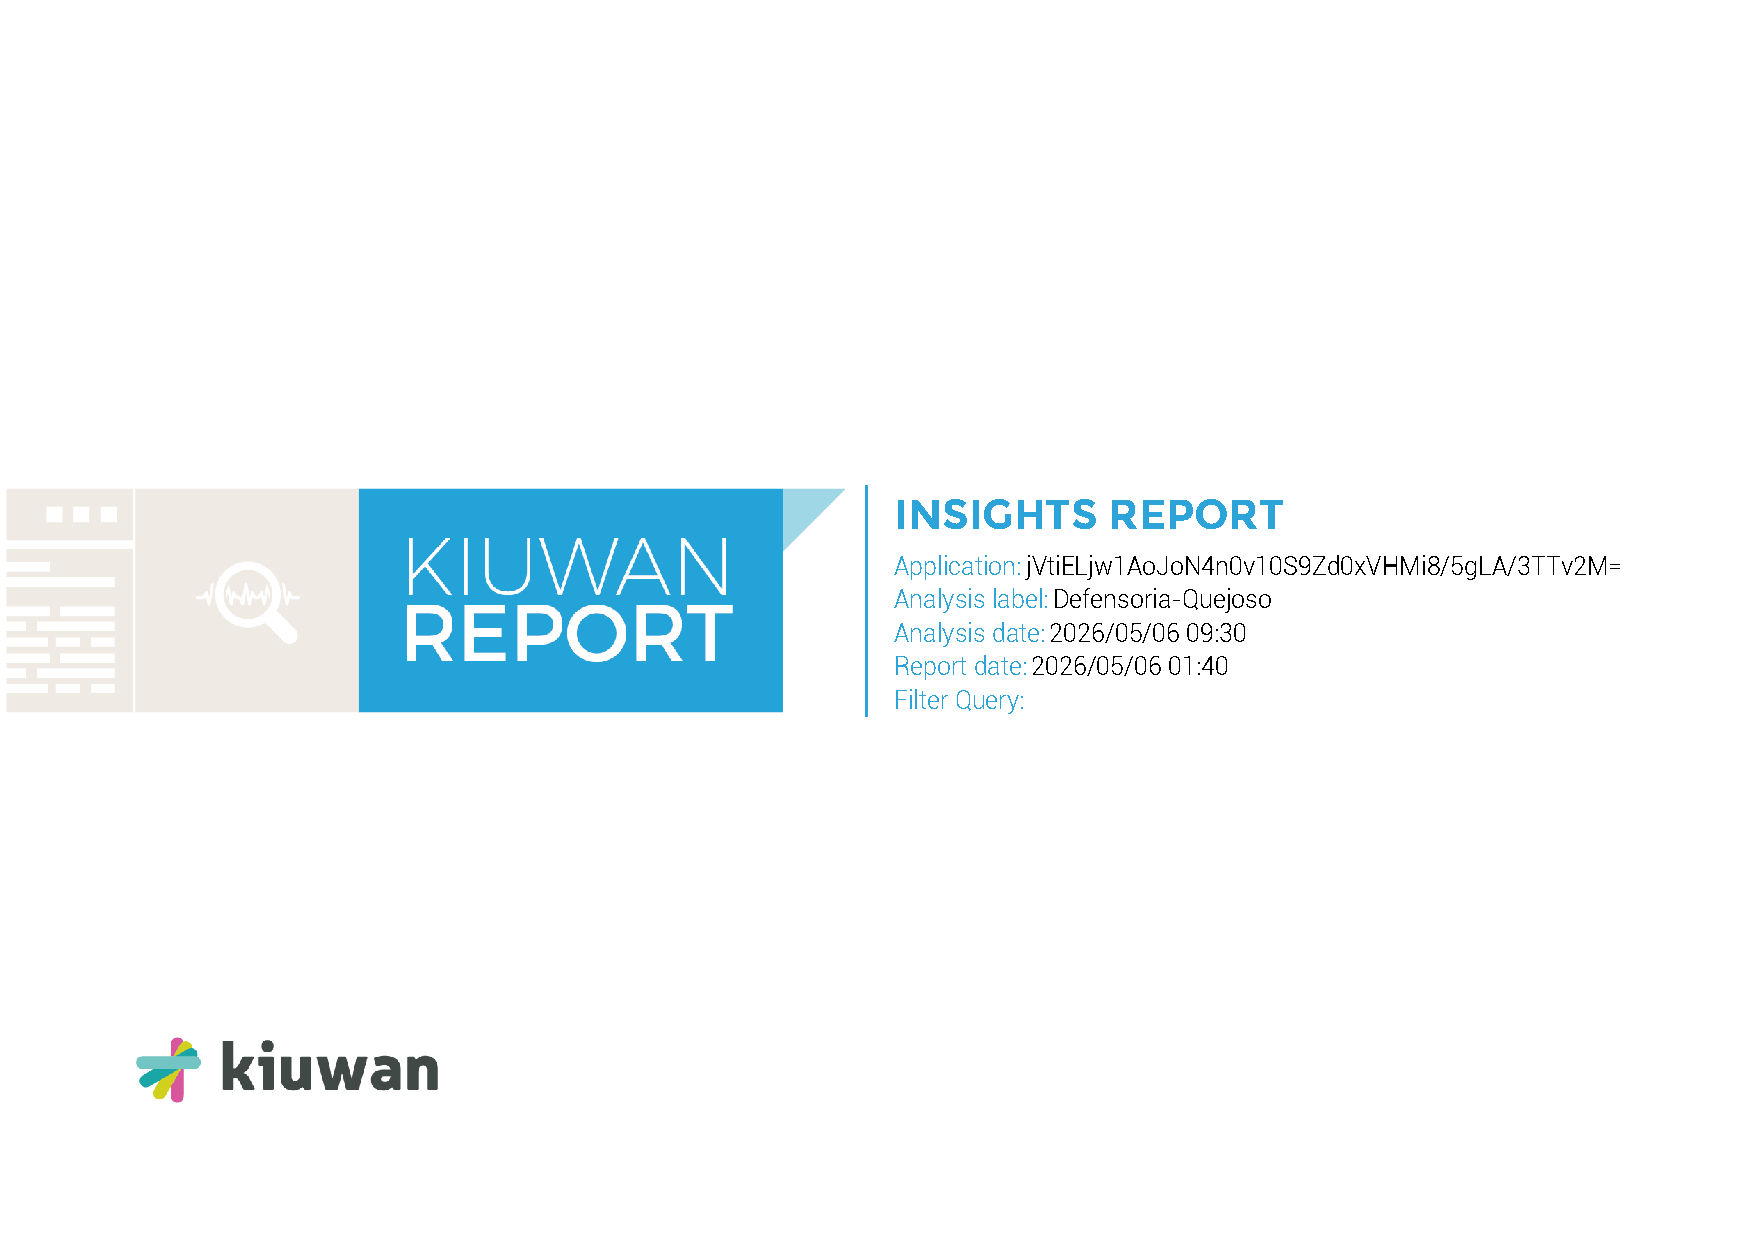
\includepdf[pages=-, frame, scale=0.8, pagecommand={\thispagestyle{plain}}]{kiuwan/quejoso/INSIGHTS_REPORT-QUEJOSO.pdf}

\section{Resumen de Seguridad de la Aplicación}
\label{anexo:quejoso_app_security}
Reporte ejecutivo que muestra la calificación de seguridad de 1 estrella y la distribución de defectos en los archivos controladores.

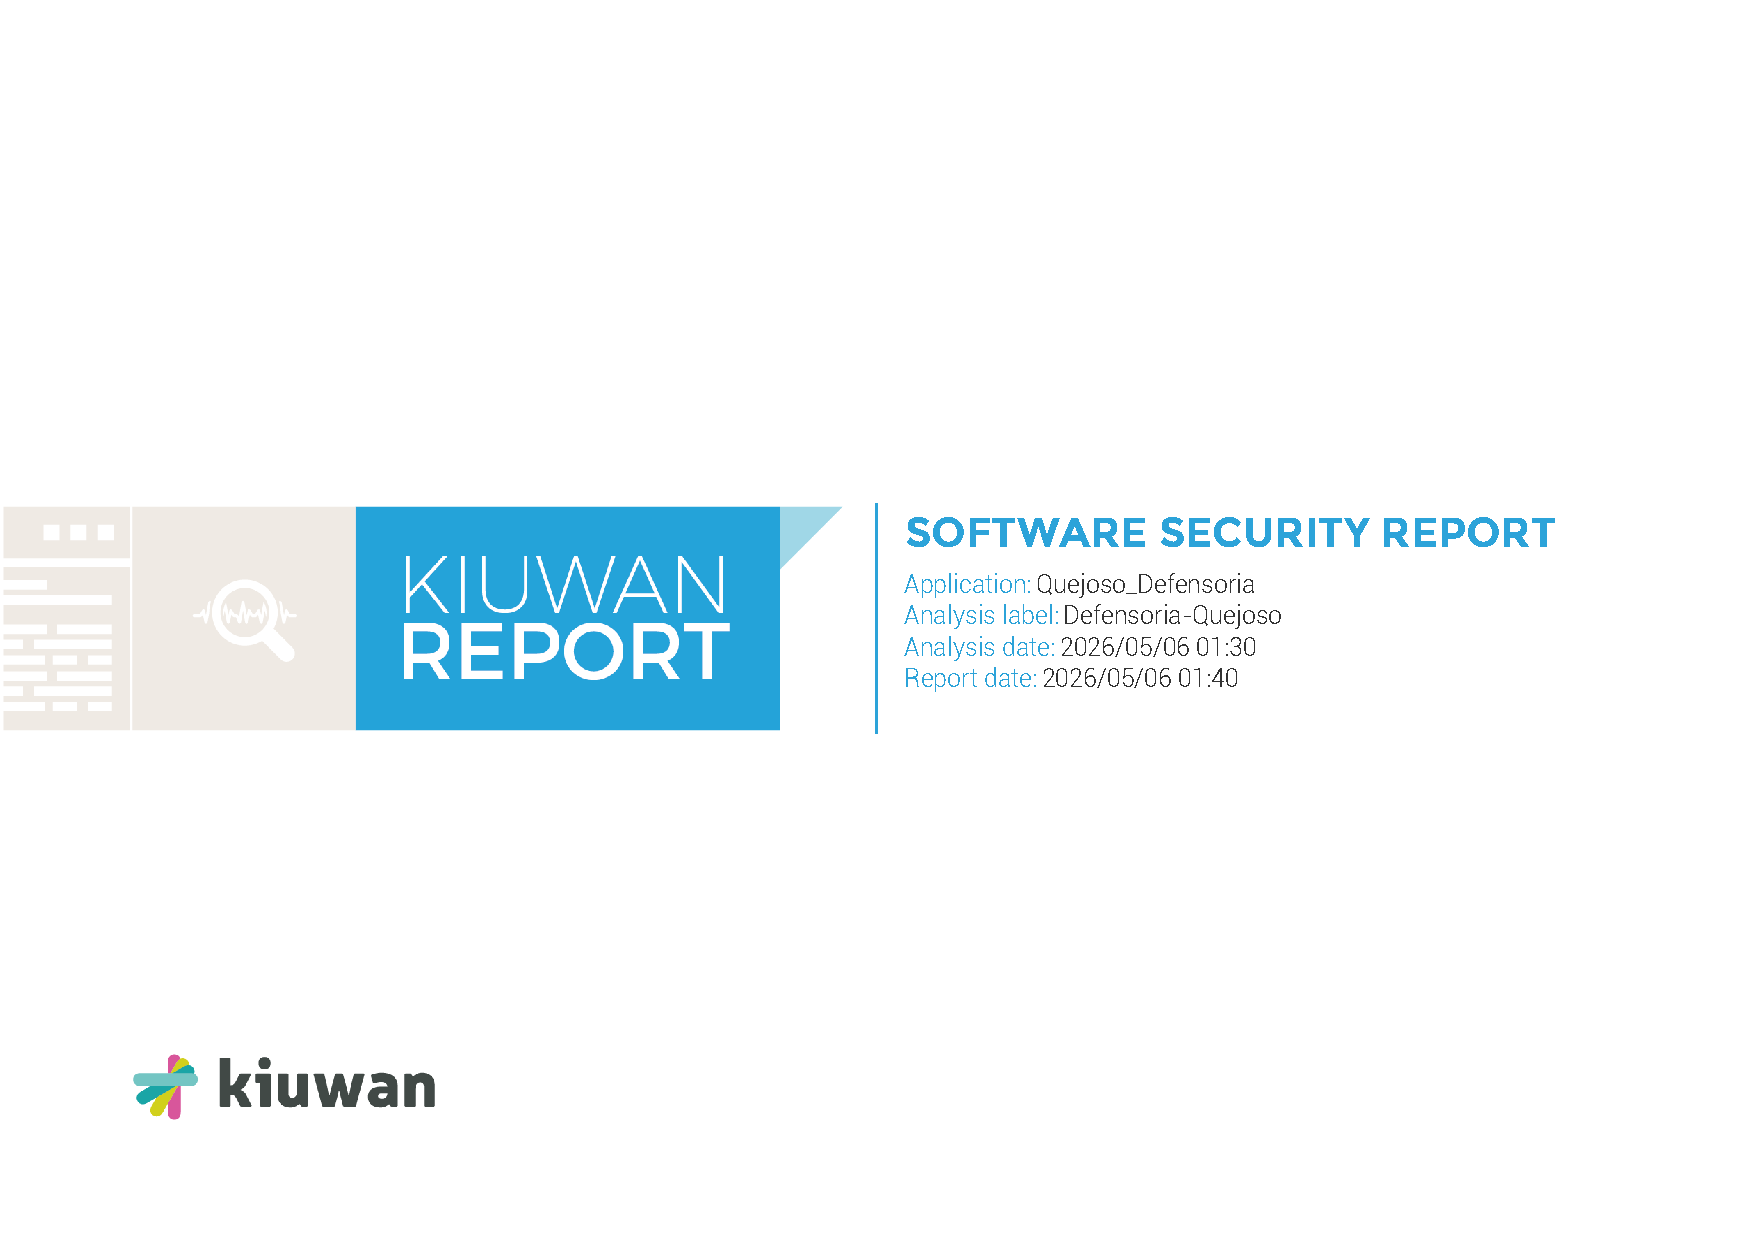
\includepdf[pages=-, frame, scale=0.8, pagecommand={\thispagestyle{plain}}]{kiuwan/quejoso/SOFTWARE_SECURITY_REPORT-QUEJOSO.pdf}